% Dokumentklassen s�ttes til memoir
\documentclass[12pt,a4paper]{report}

% Sproget s�ttes til dansk og orddeling indl�ses
\usepackage[pdfborder={0 0 0}]{hyperref}
\usepackage[latin1]{inputenc}
\usepackage[T1]{fontenc}
\usepackage[english]{babel}
\usepackage{amssymb, amsmath}
\usepackage{cite}
\usepackage{algorithmic}
\usepackage{algorithm}
\usepackage{listings}
\usepackage{enumerate}
\newcommand{\code}[1]{\texttt{#1}}

% Tabeller og s�jler
\usepackage{array, booktabs, dcolumn}
\newcolumntype{d}[1]{D{,}{,}{#1}} % Justering under komma

% Figurer
\usepackage{graphicx, caption, subfig}
\captionsetup{font=small,labelfont=bf}

\usepackage{fixme}

\newcounter{problemnr}
\newcounter{subproblemnr}
\setcounter{problemnr}{0}

\parindent 0pt
\parskip 4mm

\title{Advanced Data Structures: van Emde Boas Trees}
\author{Anders Ingemann (20052979) \and Peter E. Hvidgaard (20062546)}

\begin{document}
\maketitle

\section*{Project}
This project is about priority queues based on the Binary Heap and Fibonacci Heap respectively. The main difference is that the Fibonacci Heap have a amotized $O(1)$ \textit{decrease key} operation, where the Binary Heap have $O(\log n)$.

We will implement both heaps, and use them to implement Dijkstras Algorithm for Single Source Shortest Path. Then we will describe a class of graphs with many \textit{decrease key} operations to hopefully show that Fibonacci Heap is faster, despite the much larger constants hidden in the big-O notation.

\section*{Queue implementations}
A list in Haskell is nothing more than a singly linked list. So in other words, it's cheap to add or remove the first element, but very expensive to add an element to the tail, or remove the last element. Throughout the description of the queues, we will omit talking about trivial cases for the remove operation when we have an empty queues. This is because the only sensible action is to return nothing.

\textbf{Teoretiske overvejelser og overfladisk analyse af deres running times}

\subsection*{A standard Haskell list}
Using a standard Haskell list is a very simple data structure. Unfortunately it is only usable as a queue if you gurantee that it only contain a few elements. Because of how Haskell represent lists, when inserting at the end of the queue, it will have to traverse the entire list, before appending the new element. Thus the complexity for inserting is $O(n)$. Removing on the other hand, is fairly simple. You can simply remove the first element in constant time. Thus $O(1)$ for remove.

\subsubsection{Worst-case input}
The worst-case test is fairly straight forward. Simply insert $n$ elements and that is it.

\subsection*{A pair of lists}
Using a pair of lists, we can obtain amotized $O(1)$ as long as we do not repeat expensive operations. The queue works by having a pair lists, a $left$ and a $right$. When inserting, we will add the element to the head of $right$. Removing on the other hand is a bit more complicated. There are 2 cases:
\begin{enumerate}
	\item $left$ contain 1 or more elements.
	\item $left$ is empty and $right$ contains 1 or more elements.
\end{enumerate}
For (1), the remove operation will simply remove the head. For (2) it's a bit more involved. The list $right$ is reversed, become $left$ and the first element is removed, this makes sense, because that will be the oldest element in the queue. The running time of the insert operation is still $O(1)$, however the remove operation can be $O(n)$, especially, the first time er remove an element, we will reverse $right$. If we gurantee that we do not repeat the expensive operation, we have a $O(1)$ amotized (for every element we have in the reverse operation, we will do a remove paying for that element). However, it is common in the functional paradigm to reuse functions. Therefore one should take care to not use expensive operation more than once. This also provide us with the worst-case behaviour.

\subsubsection{Worst-case input}
Just as with the single list queue, the worst-case test is straight forward: insert $n$ elements and repeat the remove of the first element.

\subsection*{A pair of lists, exploiting laziness}
As described in the paper \textit{Simple and Efficient Purely Functional Queues and Deques} by Chris Okasaki, we can exploit lazyness to achieve the same $O(1)$ amotized bound, but with an improved worst-case to $O(\log n)$.

To achieve this, we want to calculate the reverse of $right$ in an incremental fashion, i.e. $left$ ++ rev$(right)$, where ++ is the append operation. Since append is lazy, we have to make the reverse lazy as well. To do this, we replace <$left$, $right$> with <$left$ ++ rev$(right)$, []> periodically. This is called a rotation, denoted $rot$, and is a fusion of append and reverse. The function $rot$ takes as input 3 lists, $left$, $right$ and $acc$ - it will then peel of the elements of $left$ one by one. For each element it will also take off an element from $right$ and append it to $acc$. Assuming that $left$ and $right$ have the same length, once the recursion have removed all elements from $left$, the content of $acc$ will be the reversed $right$. Because append operation is lazy, the recursive calls to $rot$ will be lazy as well.

The details of this can be found in the before mentioned paper.

The data structure works by maintaining an invariant, $|right| \leq |left|$. We maintain this invariant by calling $rot$ whenever $right$ become strictly larger than $left$, i.e. when $|right| \geq |left| + 1$. So, when inserting we make a call to $rot$ every time we have inserted $|left| +1$ elements. But the lazy nature of $rot$ means the actual evaluation will be deferred until needed. This makes insert $O(\log 1)$. When we call remove, it is possible that $left$ consists of a series of deferred $rot$ calls, all of which have to be evaluated. We know that each of those calls will reduce the size of $left$ in half, thus the recursion will have depth of $\log n$. Again the lazy nature of $rot$ ensure that only $\log n$ work will be done, giving the $O(\log n)$ bound.

\subsubsection{Worst-case input}
We have already mentioned how $left$ should be to enforce the worst-case behaviour. By inserting $1 + 2^i$ for any $i$ will leave us with such a senarios for the first time we call remove. Note, due to memoization repeating this call will not be expensive for any successive calls. This is importent when timing several runs to gain an average.

\subsection*{A $O(1)$ list}

\subsubsection{Worst-case input}
\section*{Fibonacci Heap}
om fib-heap
\section*{Primitive Priority Queue}
To test for correctness and to have some ``stupid'' reference, we implemented a very primitive queue. This queue is a linked list. \em{Initialize}, \em{insert} and \em{decrease\_key} are all constant operations. The \em{find\_min} and \em{delete\_min} operations scan the entire list and, in case of \em{find\_min}, returns the minimum element, a $O(n)$ operation.
\section*{Sorting Benchmark}

\begin{figure}[htb]
\centering
\includegraphics[width=0.8\textwidth]{../benchmark/cli/Sort_rand_ins.png}
\caption{Insert average}
\label{fig:randsort-ins}
\end{figure}

\begin{figure}[htb]
\centering
\includegraphics[width=0.8\textwidth]{../benchmark/cli/Sort_rand_dm.png}
\caption{Deletemin/tree walk averate pr node}
\label{fig:randsort-dm}
\end{figure}

\begin{figure}[htb]
\centering
\includegraphics[width=0.8\textwidth]{../benchmark/cli/Sort_rand_total.png}
\caption{Total running time}
\label{fig:randsort-tot}
\end{figure}
\section*{Results}
\subsection*{Maximizing decrease key calls}
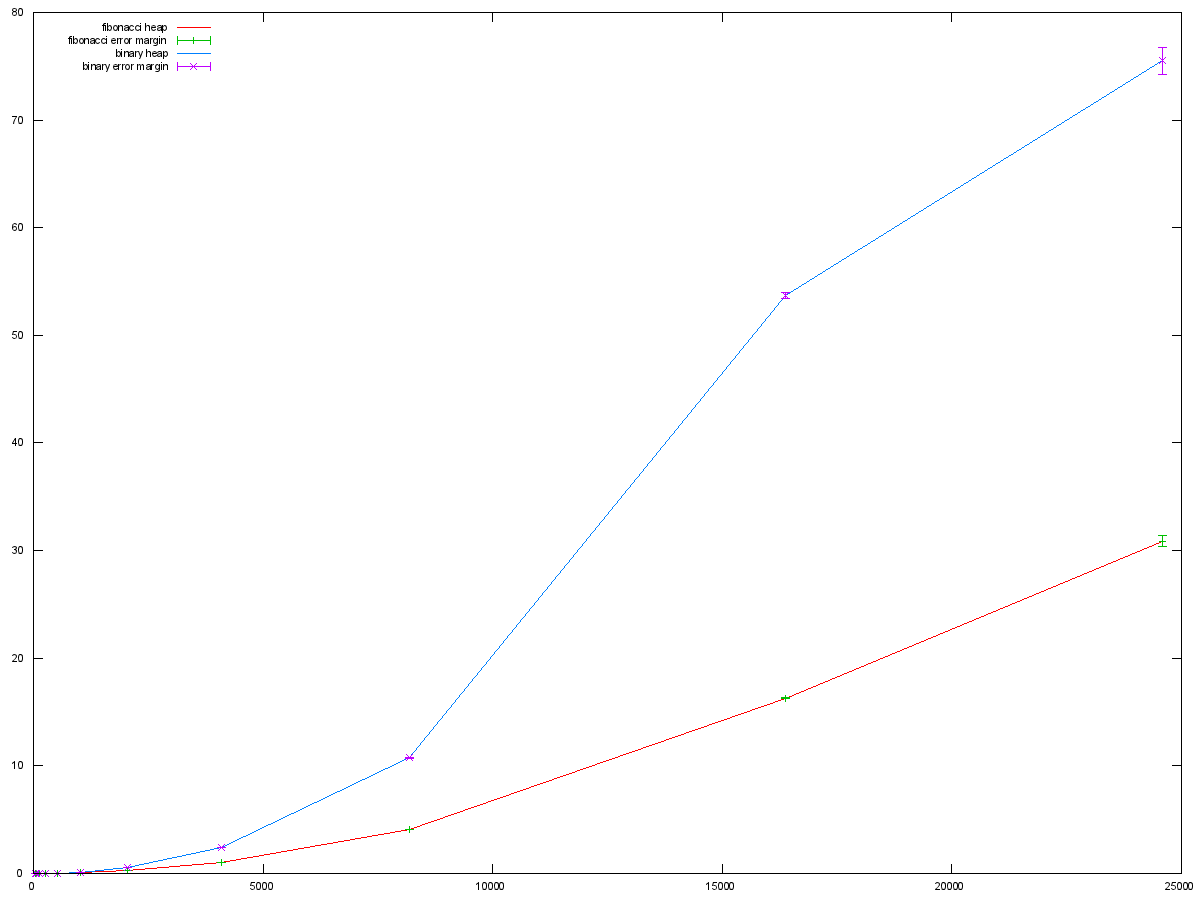
\includegraphics[scale=0.30]{../results/fibonacci-binary-dkmax2.png}
 
It's rather obvious that Binary Heap performs significantly worse than Fibonacci Heap, just as expected. The Binary Heap curve has an odd shape, but we triple checked the results, so our guess is that some underlying VM or hardware played a role, most likely page faults.
\subsection*{Random Graphs}
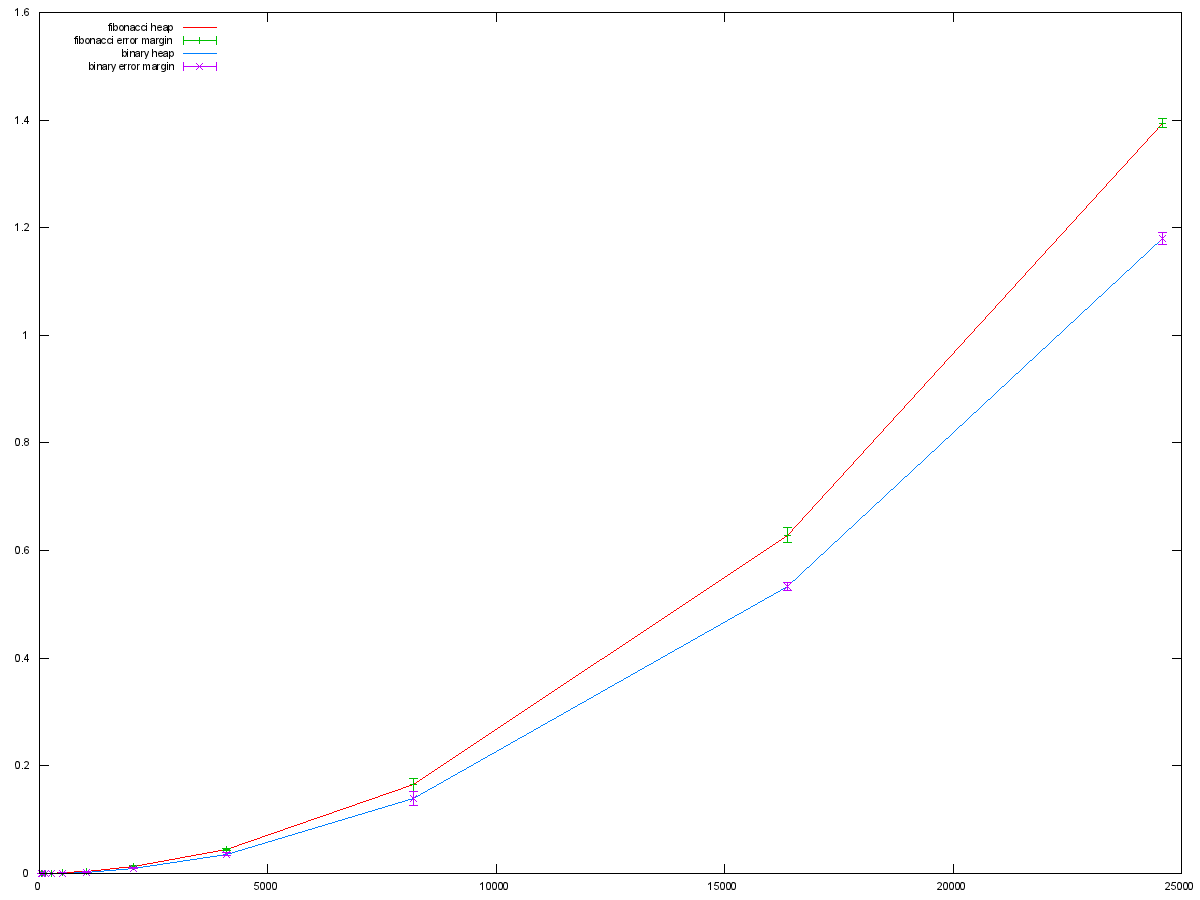
\includegraphics[scale=0.30]{../results/fibonacci-binary-random.png}

Here we see that the difference between Binary and Fibonacci heaps are almost insignificant, but with Binary Heap leading. The graphs was created with chance of edge 15\% and max weight 20.
\section*{Conclusion}
It's fairly obvious that unless given a graph, that is constructed in such a way that maximize \textit{decrease key} calls and the work the Binary Heap have to do, then then Binary Heap is to be prefered due to the much smaller constants.

\pagebreak
\begin{thebibliography}{3}

\bibitem{cormen}
Thomas H. Cormen et. al.,
\emph{Introduction to algorithms},
2nd Edition.

\end{thebibliography}

\end{document}